\chapter{The compartmental model: chronic kidney disease}
\label{applications-fits_incon_v_con}

Chronic Kidney Disease, commonly known as CKD, is the slow and
progressive loss of kidney function. There are five stages to the
disease, with the final stage being kidney failure (end-stage renal
disease--ESRD). The most common causes of CKD are diabetes and high
blood pressure.  Damage to kidneys is usually permanent, but treatment
and life style changes can slow disease
progression. \cite{_k/doqi_2002}

Since symptoms develop late in the disease, CKD progress is determined
by the level of Glomerular filtration rate (GFR), an estimate of the
flow of filtered fluid through the kidney. Patients with Stage 1 CKD
have GFR levels above 90 mL/min/1.73 m$^2$.  At this stage, kidney
damage has already begun even though GFR remains at normal levels.
Stage 2 CKD is defined as GFR between 60 and 90 mL/min/1.73 m$^2$.  At
Stage 3 CKD, a few symptoms appear with laboratory abnormalities in
other organ systems as the GFR decreases to levels between 30 and 60
mL/min/1.73 m$^2$.  When the GFR decreases to levels between 15 and 30
mL/min/1.73 m$^2$, Stage 4 CKD patients have mild symptoms and many
organ systems display lab abnormalities.  Stage 5 CKD is kidney
failure, defined as having GFR levels below 15 mL/min/1.73 m$^2$ and
not on being on renal replacement therapy, such as dialysis.  At this
stage, the kidneys no longer function and the patient needs dialysis
or a kidney transplant to survive.  There are two main types of
dialysis for kidney treatment--hemodialysis and peritoneal dialysis.
Hemodialysis filters wastes and excess fluids from the blood
externally using a machine while peritoneal dialysis uses the lining
of the peritoneal cavity and a catheter to filter wastes from the
blood. \cite{_k/doqi_2002, dipiro_pharmacotherapy:_2008}

This example focuses on ESRD dialysis patients because it has four
different types of data, shown in Figure \ref{fig:app-CKD data}.  The
majority of data are from studies or registry reports.  Countries with
a known lack of dialysis or transplantation and no other available data
used data from the Genitourinary Expert Group.  The analysis
includes a total of $5664$ data points representing $161$ countries in
all $21$ GBD 2010 study regions.  Data from Australasia is shown in 
\ref{fig:app-CKD data}.  Transplantation incidence among the prevalent
dialysis population was used as a proxy for remission.  The model
combines hemodialysis and peritoneal dialysis for analysis.

    \begin{figure}[h]
        \begin{center}
            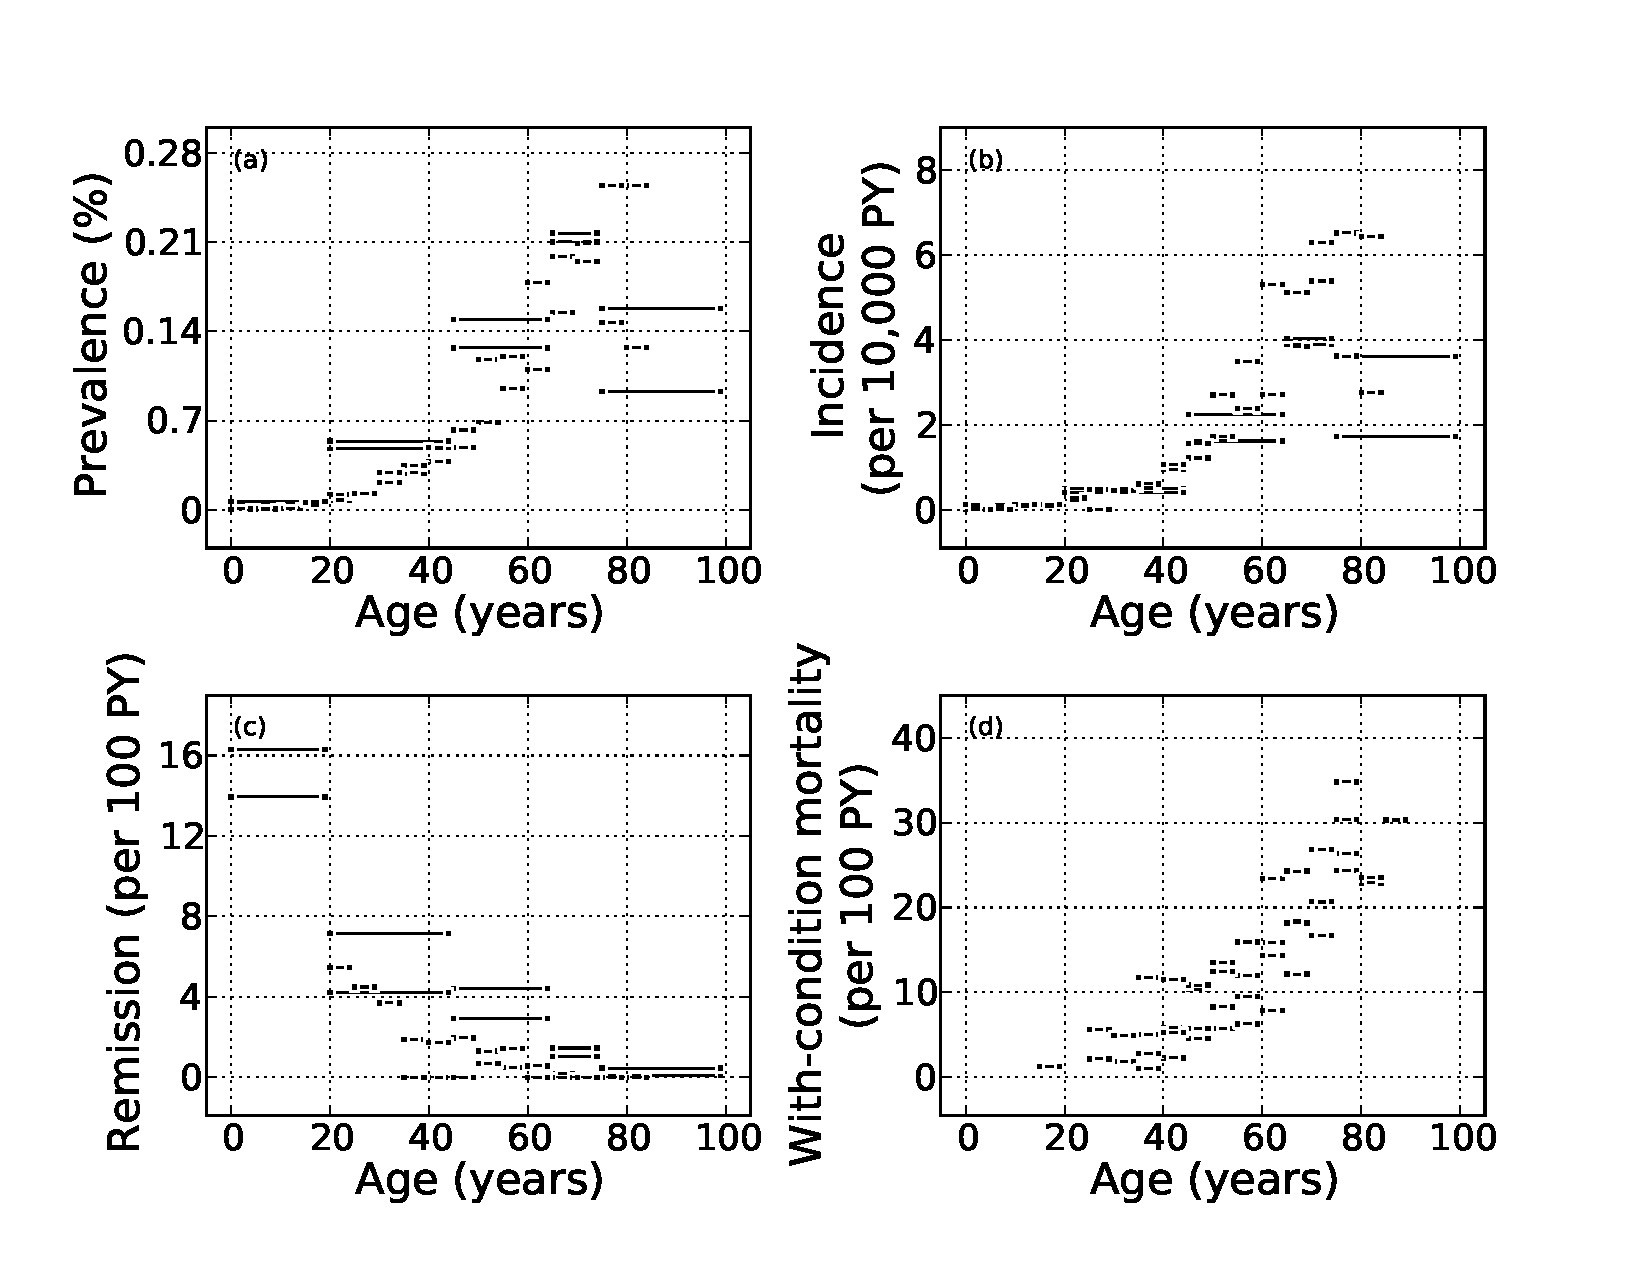
\includegraphics[width=\textwidth]{ckd-data.pdf}
            \caption{Data for 2005 Australasia ESRD dialysis has four
              data types-prevalence (panel (a)), incidence (panel
              (b)), remission (panel (c)) and with-condition mortality
              (panel (d)).}
            \label{fig:app-CKD data}
        \end{center}
    \end{figure}

As discussed in Chapter \ref{sys-dynamics}, epidemiologic parameters,
such as incidence, prevalence, remission, and with-condition
mortality, are related by a logical requirement of internal
consistency.  A prevalent case can only exist if there was a past
incidence event and the current number of prevalence cases can be
determined from past prevalent cases, new incident cases, deaths and
remissions.  Modeling the parameters simultaneously produces a best
estimate and plausible uncertainty bounds for incidence and prevalence
that are internally consistent for a single time, place and sex.

Figure \ref{fig:app-CKD incon v con} compares the compartmental and
spline model results for Australasian males with dialysis
treatment for CKD in 2005.  While the spline model estimates each
epidemiologic parameter separately, the compartmental model estimates
prevalence, incidence, remission and with-condition mortality
simultaneously.  

    \begin{figure}[h]
        \begin{center}
            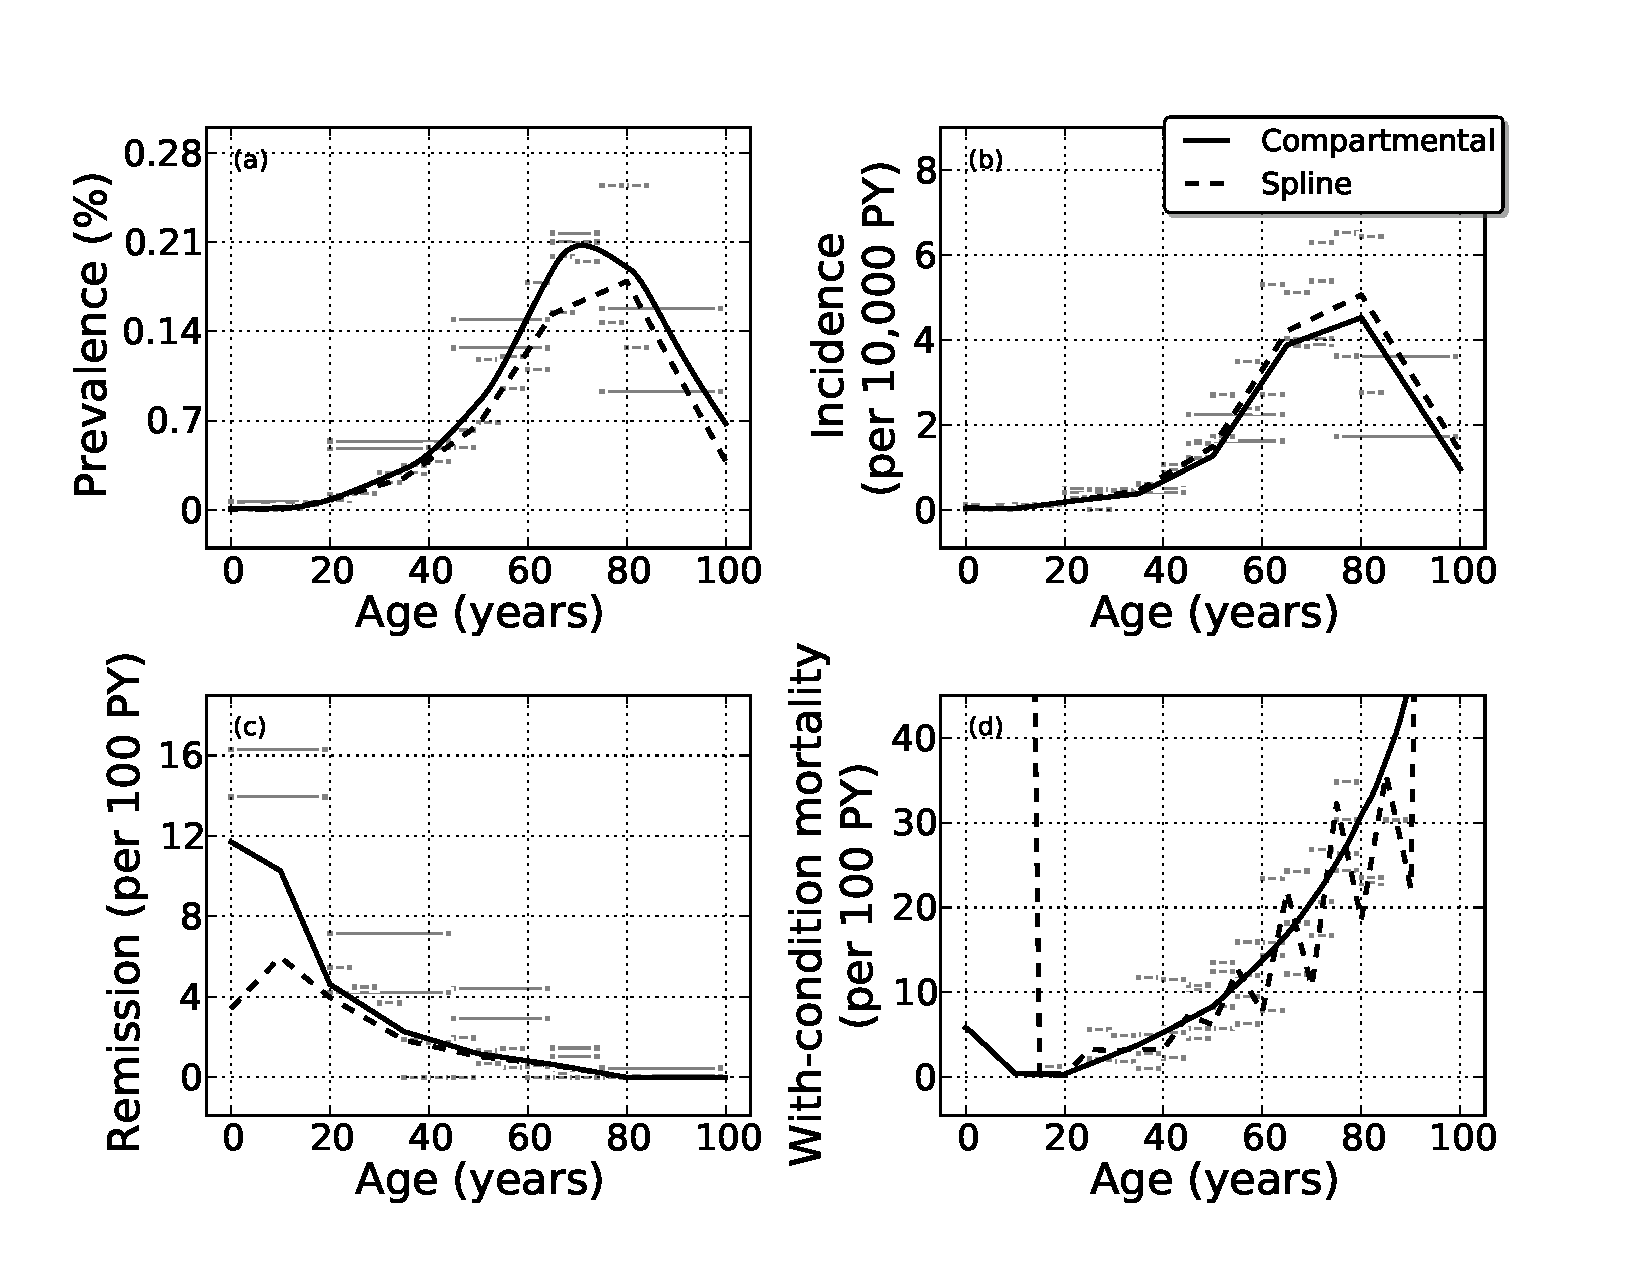
\includegraphics[width=\textwidth]{ckd-incon_v_con.pdf}
            \caption{Comparison of epidemiologic parameter estimates
              for Australasian males with dialysis treatment for CKD
              in 2005 using the compartmental and spline
              models.}
            \label{fig:app-CKD incon v con}
        \end{center}
    \end{figure}

An advantage to compartmental modeling is an estimate with a smooth
age pattern. Modeling each epidemiologic parameter individually, the
spline model follows the data exactly, often producing an
uneven age pattern as seen in Figure \ref{fig:app-CKD smooth}.  This
effect can be minimized by placing an informative prior on the
penalized spline model as discussed in Chapter
\ref{theory-age_pattern_model}.

    \begin{figure}[h]
        \begin{center}
            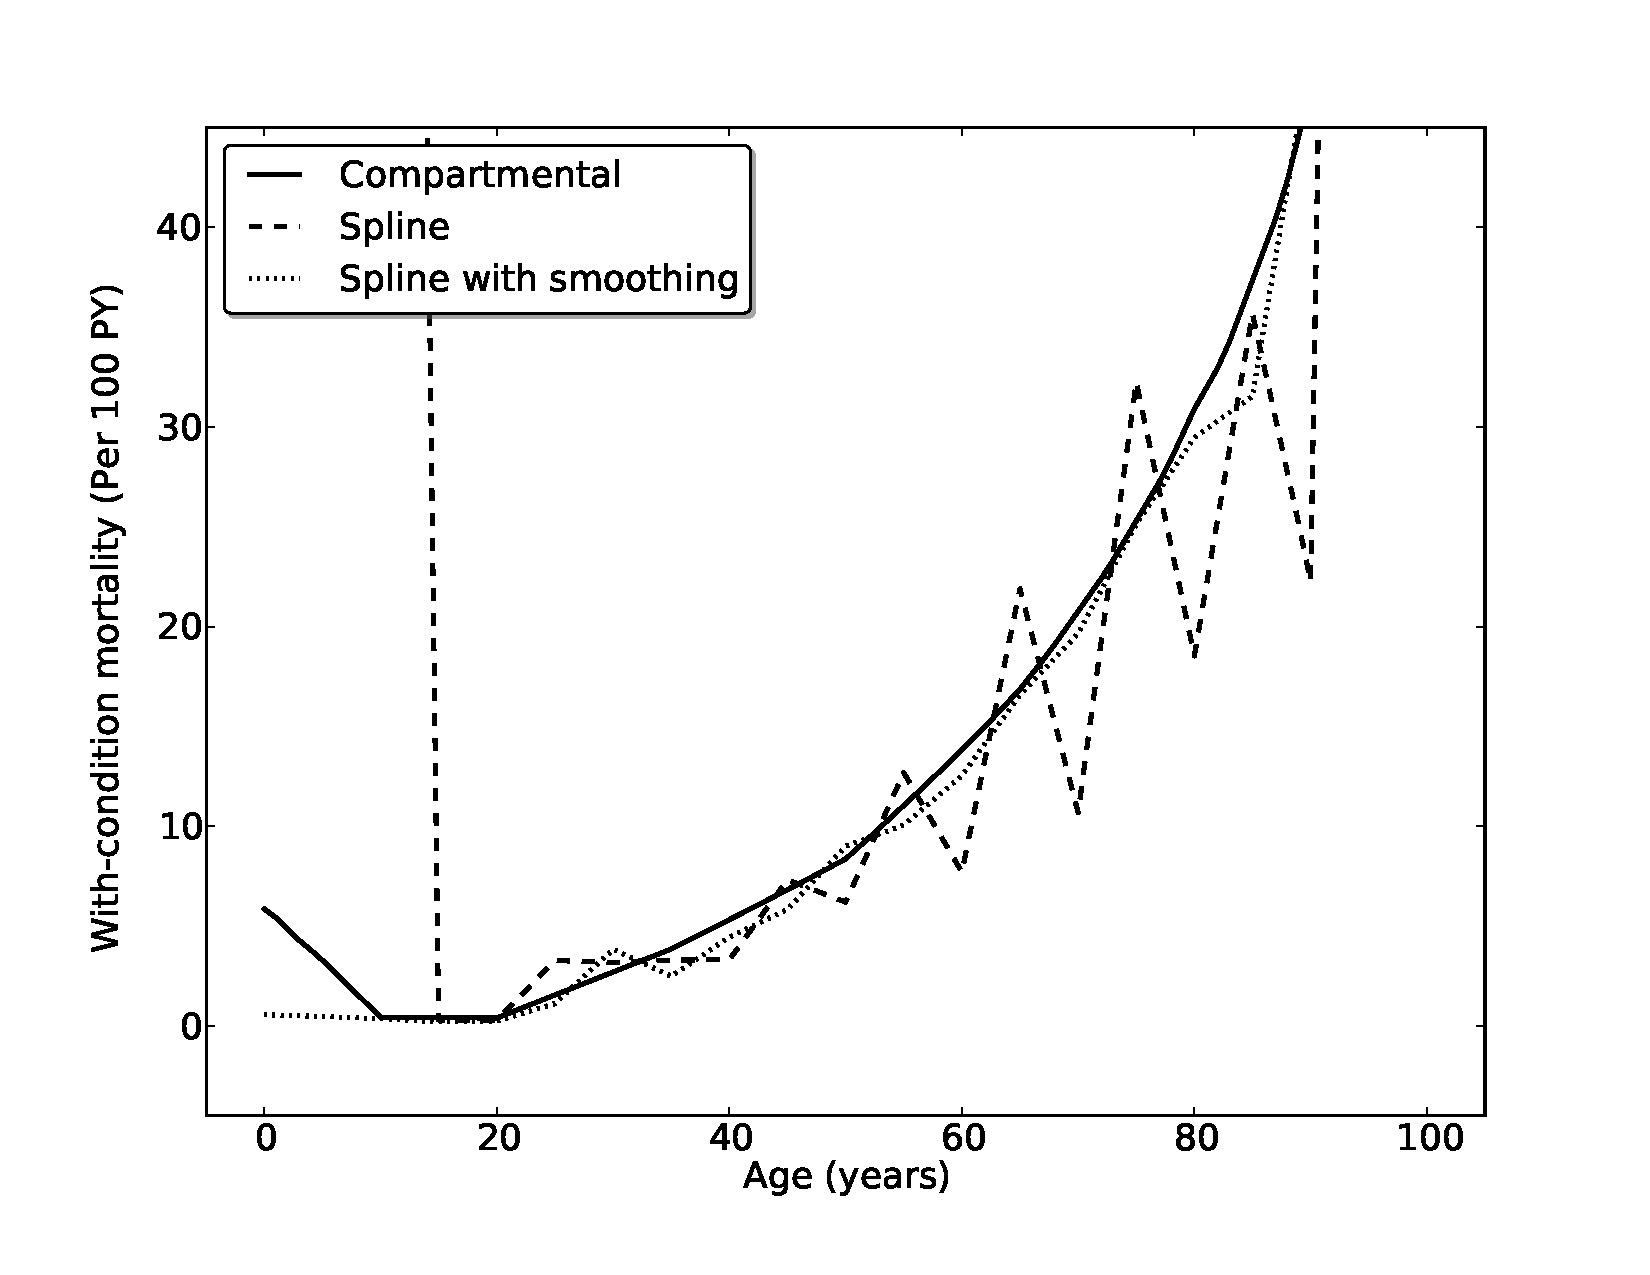
\includegraphics[width=\textwidth]{ckd-m_with_smoothing.pdf}
            \caption{With-condition mortality estimates for
              Australasian males with dialysis treatment for CKD in
              2005 using a compartmental model, spline model
              and spline model with a smoothing parameter.}
            \label{fig:app-CKD smooth}
        \end{center}
    \end{figure}

Another means of comparing the spline and compartmental
models is by a comparison of the region age-standardized prevalence
estimates.  As seen in Figure \ref{fig:app-CKD asp}, the single rate
type model produces prevalence estimates that are systematically lower
than the compartmental model because of the logic requirement that
requires all prevalence cases to have a corresponding incident event.

    \begin{figure}[h]
        \begin{center}
            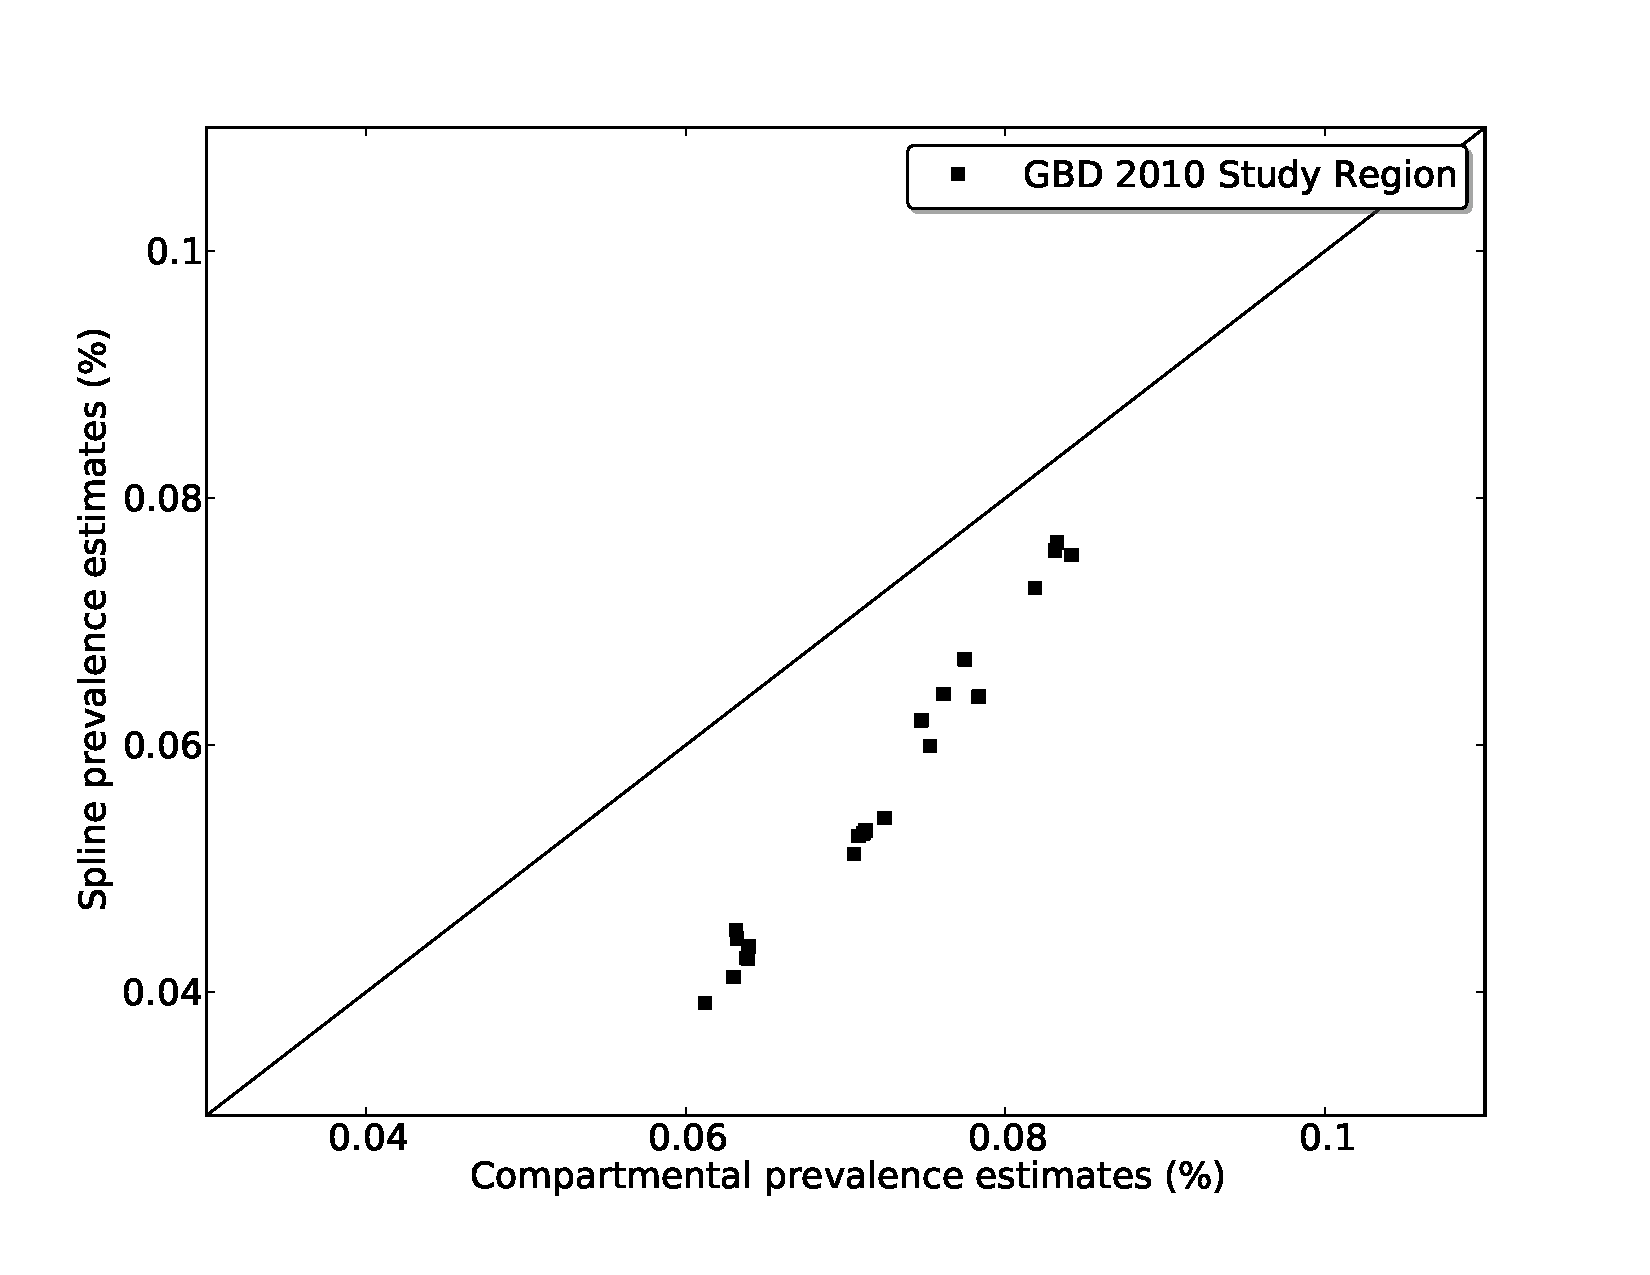
\includegraphics[width=\textwidth]{ckd-asp_scatter.pdf}
            \caption{Comparison of the regional age-standardized
              prevalence estimates using compartmental and single rate
              type models for males with dialysis treatment for CKD in
              2005.}
            \label{fig:app-CKD asp}
        \end{center}
    \end{figure}
